\chapter{Energy disaggregation assisted by appliance state sensing}\label{chap5}

In this chapter, we propose an energy disaggregation algorithm. It uses the appliance state sensor network to determine states of appliances, and uses a central energy meter to get power numbers in Watts. 

\section{Energy disaggregation algorithm}

The sensors can tell when and which appliance power state is changed. However, it has no capability of providing power consumption numbers. With the knowledge of the total power consumption trace, we are able to associate each appliance power state change (event) with the change in total consumption, so that we are able to infer the consumption of that particular appliance, assuming its consumption is stable. 

There are some challenges to do so. Firstly, there is usually slight variation in the power that an appliance takes. Some appliances have stable power traces, such as lights, others may have large variations in the power traces. We see 5W-10W variation in the power traces of laptops when browsing web pages. When there are a number of appliances, the variation adds up at the central meter, so that we usually see a very noisy power trace. Most of the appliances we use consumes tens of watts, and the variation is sometimes at the same order of magnitude. Therefore, it is hard to get the accurate power change due to an event.

Secondly, power changes observed at the central meter may not be synchronous with the events. The time difference may be several seconds. Especially when multiple events happens close in time, the power trace goes as a slope, instead of having sharp steps. 

To overcome these problems, we run piecewise constant (PWC) denoising algorithm on the central power trace first. It estimates the original signal with a piecewise constant signal which only have a small number of step changes. This process can remove the noises and detect step changes. The algorithm is discussed in the next section in detail. We can not use a lowpass filter, because the high frequency noises are in the same frequency range as the step changes. After PWC denoising, we can match the step changes with the events, according to their timestamp. If the event is single and clear, we now have its associated power number. However, if multiple events happens close to each other, they are considered overlapping, and further disaggregation is needed to get the power number for each individual event. The block diagram of the energy disaggregation algorithm is shown in Fig./ref{fig:algooverview}. 

\begin{figure}[htb]
  \centering
  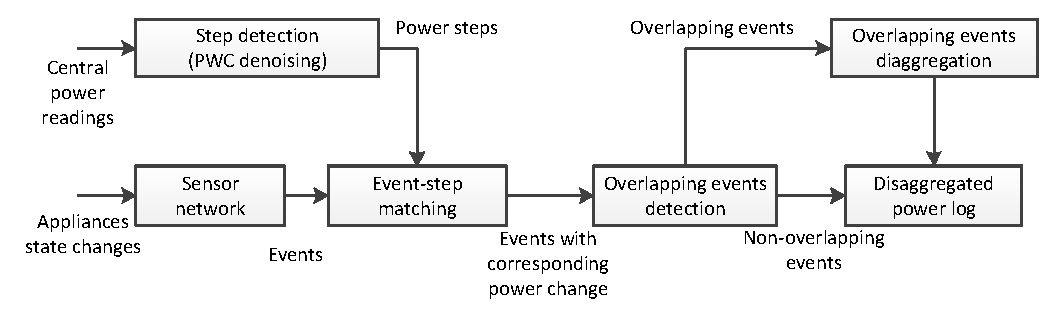
\includegraphics[width=\textwidth]{figures/algooverview}
  \caption{Block diagram of an energy disaggregation algorithm}
  \label{fig:algooverview}
\end{figure}

\section{PWC denoising and step detection in the central power trace}

In our experiments, we found that it is important to have a robust PWC denoising algorithm, especially when the number of appliance scales up and the interested appliances consumes only tens or a hundred watts. The problem is not particularly significant in previous research, because previously, people mostly focus on few appliances with very large power consumption, such as dish washers, heaters or ovens. A low pass filter is not suitable in this case because the noises have the same frequency as the step changes that we want to preserve. 

Several methods have been used in previous work to remove noise or detect step-change in the power trace. In \cite{Hart1992}, the author developed an edge detection algorithm. It looks for stable periods within the signal with variation less than a threshold (15W or VAR). The method works only when the step changes are much larger than the variation, which is not true in our case. In \cite{Norford1996}, the authors use a median filter to remove spikes in the raw signal. Total variation denoising is used in \cite{Kolter2012}. The method can effectively remove noises in the signal and preserve steps. However, its purpose is not step detection. Hence, its output is not guaranteed to be piecewise constant. 

A method called jump penalization is introduced in \cite{Little2011}. The original method is an offline one. The algorithm begins with a constant signal that estimates the input signal, which is usually the mean or median value of the input signal. In each iteration, a greedy search tries to insert a best new step-change in the current estimation. The algorithm ends when the improvement of estimation accuracy by inserting new step-changes is too small. The algorithm guarantees piecewise constant output, and the step-changes are explicitly found in each iteration. 

We adopted the algorithm to an online version, which can process the data in real time.  Instead of inserting step-changes iteratively, we insert just one step-change from the last step-change to the current sample. The flow chart of our step-detection algorithm is shown in Fig.\ref{fig:pwc}. The error function is defined as following: \[E(x,y) = \frac{1}{2} \sum_n \left(x_n - y_n\right)^2\]

\begin{figure}[htb]
  \centering
  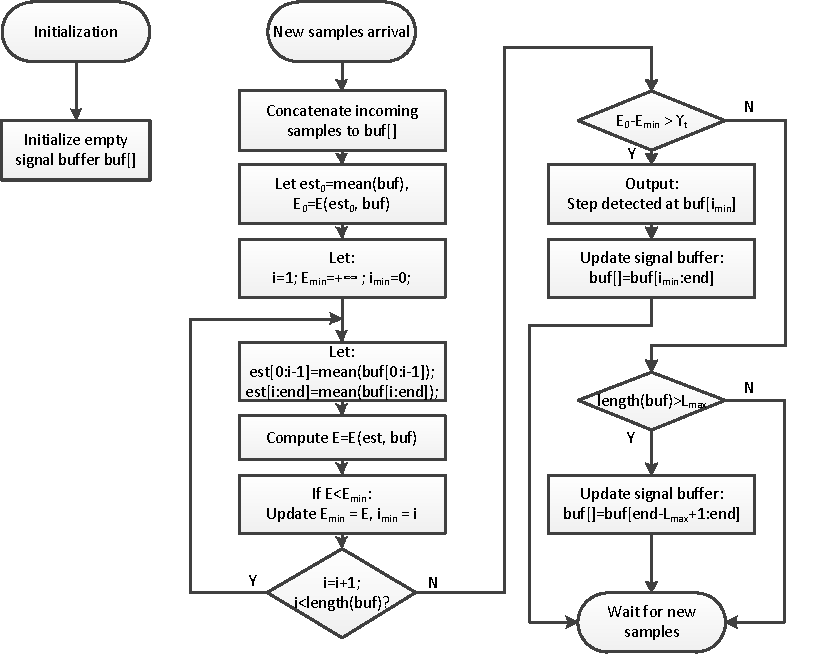
\includegraphics[width=\textwidth]{figures/pwc}
  \caption{Modified jump penalization algorithm for step detection}
  \label{fig:pwc}
\end{figure}

The parameter $\gamma$ acts as a threshold in the algorithm, or 'penalty' to insert a new step-change. With a lower $\gamma$, the algorithm is more likely to detect steps. We use a time-variant $\gamma_t$ based on our knowledge about events. When there are events detected by the sensor network, we use the lower $\gamma_l$ so that it is more likely to detect small step changes. When no events are detected, we use the higher $\gamma_h$ to reduce false steps. In practice, when the power signal is in kW, we choose $\gamma_l = 0.0001$ and $\gamma_h=0.0025$. 

We also limit the length of signal buffer to $L_{max}$, so that the greedy search domain is limited to the last $L_{max}$ samples. Otherwise, the buffer can grow indefinitely when there is no step-change in a very long time. 



\section{Experimental results}


